\documentclass[tikz,border=6pt]{standalone}
\usepackage{pgfplots}
\pgfplotsset{compat=1.18}
\usepgfplotslibrary{colormaps}
\usetikzlibrary{arrows, arrows.meta, calc}
\usetikzlibrary{decorations.markings}


\usepackage{amssymb,amsmath,mathtools}

\usepackage[T1]{fontenc}
\usepackage[utf8]{inputenc}
\usepackage{newpxtext,newpxmath}
\usepackage{sectsty}

\renewcommand{\Re}{\operatorname{\mathrm{Re}}}
\renewcommand{\Im}{\operatorname{\mathrm{Im}}}

\begin{document}
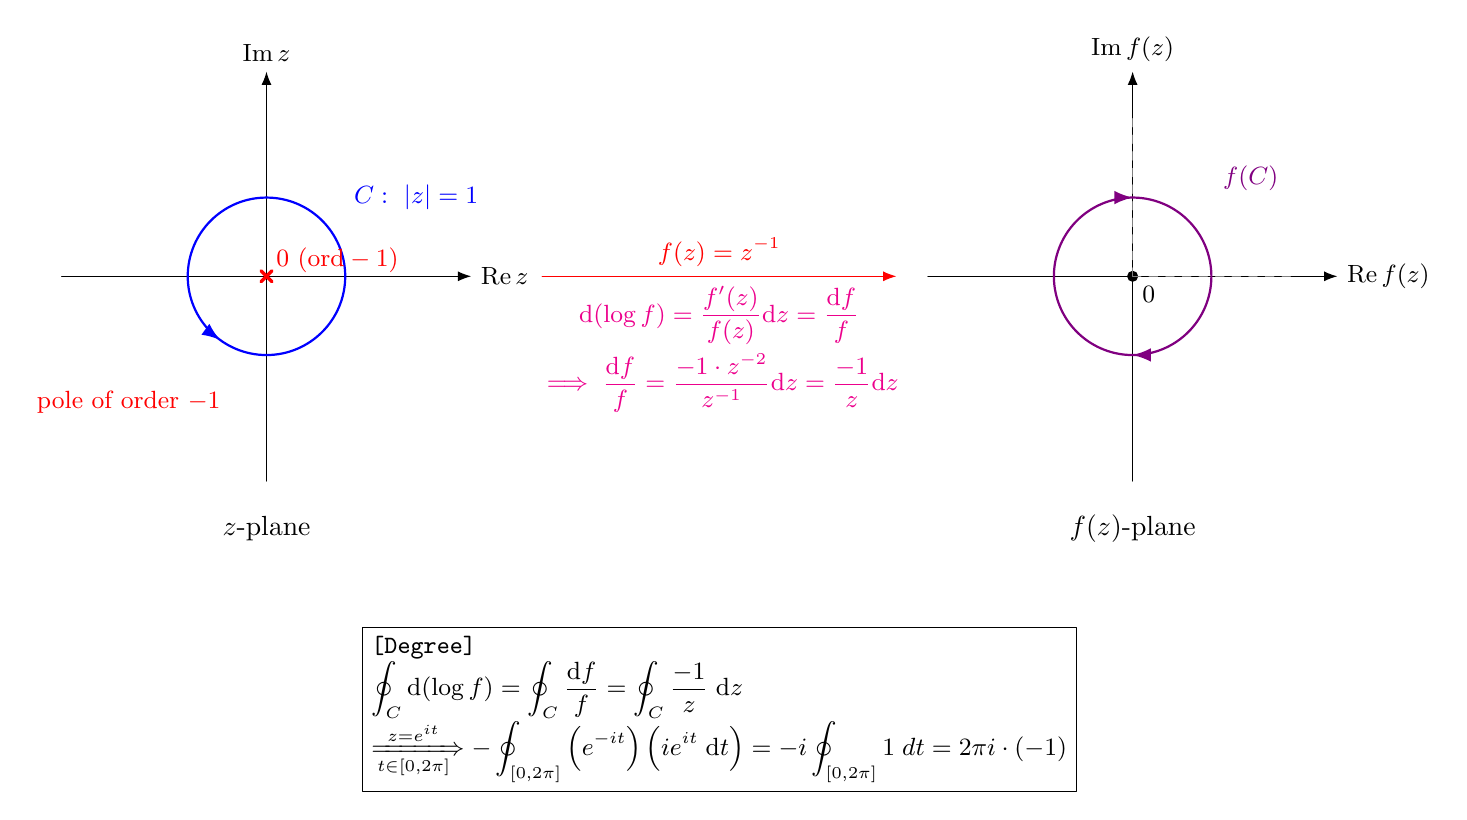
\begin{tikzpicture}[>=Latex, line cap=round, line join=round, font=\small]
%========================
% Left: z-plane
%========================
\begin{scope}[shift={(0,0)}]
	\node[font=\normalsize] at (0,-3.2) {$z$-plane};
	% axes
	\draw[->] (-2.6,0)--(2.6,0) node[right] {$\Re z$};
	\draw[->] (0,-2.6)--(0,2.6) node[above] {$\Im z$};
	% unit circle C (positively oriented) -- radius 1.5 for visibility
	\draw[blue,thick,postaction={decorate},
	decoration={markings, mark=at position 0.65 with {\arrow{>}}}]
	(0,0) circle (1);
	\node[blue] at (1.9,1.0) {$C:\ |z|=1$};
	
	% pole at 0 (order -1)
	\draw[red,very thick] (0,0) ++(-0.07,-0.07) -- ++(0.14,0.14);
	\draw[red,very thick] (0,0) ++(-0.07,0.07)  -- ++(0.14,-0.14);
	\node[red, right] at (0,0.2) {$0$ ($\mathrm{ord} -1$)};
	\node[red] at (-1.75,-1.6) {pole of order $-1$};
	
%	% function label + order via winding form
%	\node[align=left] at (0,-2.7) {$\displaystyle
%			f(z)=\frac{1}{z},\quad
%			\operatorname{ord}_{0} f
%			=\operatorname{Res}\!\left(\frac{f'}{f},0\right)
%			=\frac{1}{2\pi i}\!\oint_C \frac{-1}{\,z\,}\,dz
%			=-1.$};
\end{scope}

% function label
\draw[->, red] (3.5,0) -- (8,0) node[midway, above, align=center] {$\displaystyle
	f(z)=z^{-1}$};
\draw[->, magenta, opacity=0] (3.5,0) -- (8,0) node[midway, below, align=center, opacity=1] {
	$\displaystyle\mathrm{d}(\log f)=\frac{f'(z)}{f(z)}\mathrm{d}z=\frac{\mathrm{d}f}{f}$\\ [2pt]
	$\displaystyle\implies\frac{\mathrm{d}f}{f}=\frac{-1\cdot z^{-2}}{z^{-1}}\mathrm{d}z=\frac{-1}{z}\mathrm{d}z$};

\node[draw=black, align=left] at (5.75,-5.5) {
	\texttt{[Degree]}\\
	$\displaystyle
	\oint_C \mathrm{d}(\log f)=\oint_C \frac{\mathrm{d}f}{f}=\oint_C \frac{-1}{z}\; \mathrm{d}z$ \\
	$\displaystyle\xRightarrow[{t\in[0,2\pi]}]{z=e^{it}}-\oint_{[0,2\pi]}\left(e^{-it}\right)\left(ie^{it}\; \mathrm{d}t\right)=-i\oint_{[0,2\pi]}1\; dt=2\pi i\cdot (-1)$
%	\\ [10pt]
%	\texttt{[Coefficient]}\\
%	$\displaystyle a_0=\frac{f(0)}{0!}=\frac{1}{2\pi i}\!\oint_C \frac{f(\zeta)}{\zeta}\,d\zeta=0$ \\
%	$\displaystyle a_1=\frac{f'(0)}{1!}=\frac{1}{2\pi i}\!\oint_C \frac{f(\zeta)}{\zeta^{2}}\,d\zeta=1$\\
%	$a_n= 0$ for $n\geq 2$
	};

%========================
% Right: f(z)-plane
%========================
\begin{scope}[shift={(11,0)}]
	\node[font=\normalsize] at (0,-3.2) {$f(z)$-plane};
	% axes
	\draw[->] (-2.6,0)--(2.6,0) node[right] {$\Re f(z)$};
	\draw[->] (0,-2.6)--(0,2.6) node[above] {$\Im f(z)$};
	% origin
	\fill (0,0) circle(2pt) node[below right] {$0$};
	
	% image curve f(C): z = 1.5 e^{it} -> w = (1/1.5) e^{-it}
	% Re w = (1/1.5) cos t,  Im w = -(1/1.5) sin t  (clockwise winding)
	\draw[violet,thick,
	postaction={decorate},
	decoration={markings,
			mark=at position 0.25 with {\arrow{>}},
			mark=at position 0.75 with {\arrow{>}}}]
	plot[domain=0:6.283, samples=500]
	({ (1/1)*cos(\x r) },{ -(1/1)*sin(\x r) });
	\node[violet] at (1.5,1.25) {$f(C)$};
	
	% dashed rays to visualize winding
	\draw[gray,dashed] (0,0) -- (2.1,0);
	\draw[gray,dashed] (0,0) -- (0,2.1);
	
%	% annotation: Laurent/Taylor(-like) coefficients via Cauchy integrals
%	\node[align=center] at (0,-2.45)
%	{$\displaystyle
%			f(z)=\frac{1}{z}=\sum_{n=-\infty}^{\infty} c_n z^n,\quad
%			c_n=\frac{1}{2\pi i}\!\oint_C \frac{f(\zeta)}{\zeta^{\,n+1}}\,d\zeta.$\\[4pt]
%			For $f(z)=1/z$: $c_{-1}=\frac{1}{2\pi i}\!\oint_C \frac{1}{\zeta}\,d\zeta=1,\quad
%			c_n=0\ (n\neq-1).$\\[6pt]
%			$\mathrm{wind}\big(f(C),0\big)=-1
%			\ \Rightarrow\
%			\displaystyle \oint_C \frac{f'(z)}{f(z)}\,dz=-2\pi i.$};
\end{scope}

%		%========================
%		% Left: z-plane
%		%========================
%		\begin{scope}[shift={(0,0)}]
%			\node[font=\normalsize] at (0,3.2) {$z$-plane};
%			% axes
%			\draw[->] (-2.2,0)--(2.2,0) node[right] {$\Re z$};
%			\draw[->] (0,-2.2)--(0,2.2) node[above] {$\Im z$};
%			
%			% unit circle C (positively oriented) -- radius 1.5 for visibility
%			\draw[blue,thick,postaction={decorate},
%			decoration={markings, mark=at position 0.65 with {\arrow{>}}}]
%			(0,0) circle (1.5);
%			\node[blue] at (1.9,1.0) {$C:\ |z|=1$};
%			
%			% pole at 0 (order -1)
%			\draw[red,very thick] (0,0) ++(-0.07,-0.07) -- ++(0.14,0.14);
%			\draw[red,very thick] (0,0) ++(-0.07,0.07)  -- ++(0.14,-0.14);
%			\node[red] at (0.35,0.2) {$0$};
%			\node[red] at (-1.75,-1.6) {pole of order $-1$};
%			
%			% function label + order via winding form
%			\node[align=left] at (0,-2.7) {$\displaystyle
%				f(z)=\frac{1}{z},\quad
%				\operatorname{ord}_{0} f
%				=\operatorname{Res}\!\left(\frac{f'}{f},0\right)
%				=\frac{1}{2\pi i}\!\oint_C \frac{-1}{\,z\,}\,dz
%				=-1.$};
%		\end{scope}
%		
%		%========================
%		% Right: w-plane = f(z)-plane
%		%========================
%		\begin{scope}[shift={(7.2,0)}]
%			\node[font=\normalsize] at (0,3.2) {$w=f(z)$-plane};
%			% axes
%			\draw[->] (-2.6,0)--(2.6,0) node[right] {$\Re w$};
%			\draw[->] (0,-2.6)--(0,2.6) node[above] {$\Im w$};
%			
%			% origin
%			\fill (0,0) circle(2pt) node[below right] {$0$};
%			
%			% image curve f(C): z = 1.5 e^{it} -> w = (1/1.5) e^{-it}
%			% Re w = (1/1.5) cos t,  Im w = -(1/1.5) sin t  (clockwise winding)
%			\draw[violet,thick,
%			postaction={decorate},
%			decoration={markings,
%				mark=at position 0.25 with {\arrow{>}},
%				mark=at position 0.75 with {\arrow{>}}}]
%			plot[domain=0:6.283, samples=500]
%			({ (1/1.5)*cos(\x r) },{ -(1/1.5)*sin(\x r) });
%			\node[violet] at (1.8,1.7) {$f(C)$};
%			
%			% dashed rays to visualize winding
%			\draw[gray,dashed] (0,0) -- (2.1,0);
%			\draw[gray,dashed] (0,0) -- (0,2.1);
%			
%			% annotation: Laurent/Taylor(-like) coefficients via Cauchy integrals
%			\node[align=center] at (0,-2.45)
%			{$\displaystyle
%				f(z)=\frac{1}{z}=\sum_{n=-\infty}^{\infty} c_n z^n,\quad
%				c_n=\frac{1}{2\pi i}\!\oint_C \frac{f(\zeta)}{\zeta^{\,n+1}}\,d\zeta.$\\[4pt]
%				For $f(z)=1/z$: $c_{-1}=\frac{1}{2\pi i}\!\oint_C \frac{1}{\zeta}\,d\zeta=1,\quad
%				c_n=0\ (n\neq-1).$\\[6pt]
%				$\mathrm{wind}\big(f(C),0\big)=-1
%				\ \Rightarrow\
%				\displaystyle \oint_C \frac{f'(z)}{f(z)}\,dz=-2\pi i.$};
%		\end{scope}
\end{tikzpicture}
\end{document}






